\problemname{Upplega}

\begin{center}
  \textit{``It's beginning to look a lot like Christmas\\ Everywhere you go''}
\end{center}
  
\noindent
It is only truly winter once the snow has settled on all the branches of the $N$ trees on the street outside your house.
The street with all the trees can be represented in an arbitrarily large grid. Along the street, the $N$ trees stand in a row.
The trunk of each tree $i$ is located at position $pos_i$ and is described by a rectangle with a width of $1$, occupying the
entire column $pos_i$. Additionally, each tree $i$ has $s_i$ branches. Each branch is described by a rectangle with a height of $1$ 
that sticks out from the trunk and is an integer number of units wide.
It is guaranteed that the squares that each branch occupies do not contain any other branch or trunk. It is also guaranteed that
no branch goes beyond another tree, not even above it.

After a snowy evening, Upplega has settled on all the trees.
Upplega is the Swedish term for snow that has accumulated on top of a tree's branches.
On each unit length of each branch, there is $1$ unit of snow. The snow is so small that it does not occupy a square. In other words, 
the height is negligible. 

You are a true winter enthusiast who loves Christmas songs, the cozy cold weather, and above all, all the Upplega.
According to the weather forecast, there will soon be a big storm that will shake all the trees quite vigorously.
When a tree is shaken, the snow on its branches will start falling straight down until the snow either safely lands
on a branch belonging to a tree that is not shaking, or lands on the ground.

Despite the storm approaching, you have time to protect $K$ trees from shaking by rooting them.
Since you love snow so much, you want to calculate the maximum number of snow units you can prevent from falling
to the ground by rooting exactly $K$ trees.

\begin{centering}
  \begin{figure}[h]
      \centering
      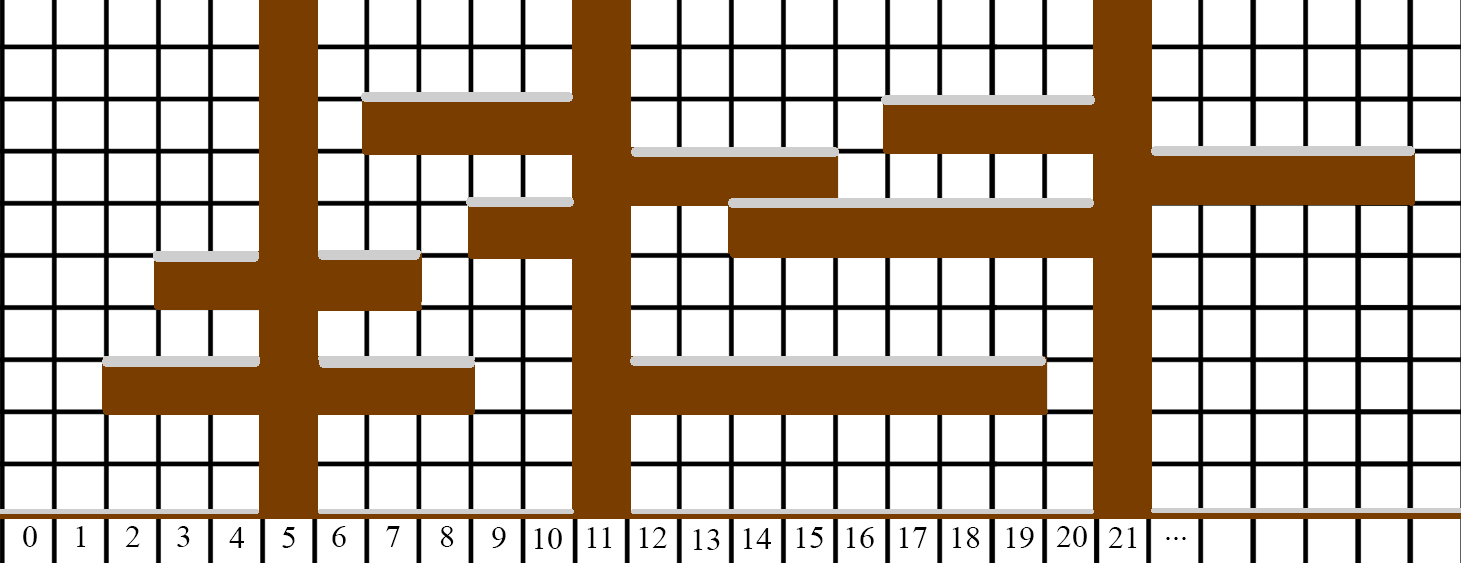
\includegraphics[width=0.8\textwidth]{sample1.png}
      \caption{The picture shows sample 1.}
  \end{figure}
\end{centering}

\section*{Input}
\noindent
The first row of input contains two integer $N$ and $K$ ($1 \leq K \leq N \leq 10^5$), the number of
trees on the street and the number trees you have time to protect from being shaken.

The second row contains $N$ integers $pos_1, pos_2, \dots, pos_N$ ($0 \leq pos_i \leq 10^9$), where
$pos_i$ is the number of length units from the start of the street to tree $i$.
The trees will be given in sorted order and it is guaranteed that no two trees occupy the same position.
Formally, this means that for all $i<j$, it holds that $pos_i < pos_j$.

The third line contains $N$ integers $s_1, s_2, \dots, s_N$ ($1 \leq s_i \leq 10$), where $s_i$ is the
number of branches on tree $i$.

Finally, $2N$ rows follows, with $2$ rows per tree, which describes its branches:
\begin{itemize}
  \item The first row contains $s_i$ integers $h_{i,1}, h_{i,2}, \dots, h_{i,s_i}$ ($1 \leq h_{i,j} \leq 10^9$), where $h_{i,j}$ is the height of the $j$:th branch belonging to tree $i$.
  \item The second row contains $s_i$ integers $l_{i,1}, l_{i,2}, \dots, l_{i,s_i}$ ($-10^9 \leq l_{i,j} \leq 10^9$ , $l_{i,j} \neq 0$). 
  Each $l_{i,j}$ describes the length and direction of the $j$:th branch of tree $i$. If $l_{i,j}$ is positive, it means that branch $j$ is directed to the right and is $l_{i,j}$ length units long. 
  If $l_{i,j}$ is negative, the branch is directed to the left and is $|l_{i,j}|$ length units long.
\end{itemize}

No branch will be outside the beginning of the street located at $0$, or beyond $10^9$ length units from the beginning of the street.

\section*{Output}
\noindent
Print the maximum number of snow units that you can prevent from falling to the ground by rooting exactly $K$ trees.

\section*{Scoring}
Your solution will be tested on a set of test groups, each worth a number of points. 
Each test group contains a set of test cases. 
To get the points for a test group you need to solve all test cases in the test group.

\noindent
\begin{tabular}{| l | l | p{12cm} |}
  \hline
  \textbf{Group} & \textbf{Point value} & \textbf{Constraints} \\ \hline
  $1$    & $5$        & All branches are directed to the right. Formally, $l_{i,j} > 0$ holds for all $i,j$.  \\ \hline
  $2$    & $5$        & $K = 1$ \\ \hline
  $3$    & $7$        & $N \leq 15$ \\ \hline
  $4$    & $11$       & $N \leq 2000, |l_{i,j}| \leq 2 \cdot 10^5, pos_i \leq 2 \cdot 10^5$ for all $i,j$. \\ \hline %2000 or 1000 depending on how fast Python can solve it
  $5$    & $23$       & $N \leq 2000$  \\ \hline
  $6$    & $31$       & $ |l_{i,j}| \leq 2 \cdot 10^5, pos_i \leq 2 \cdot 10^5$ for all $i,j$. \\ \hline
  $7$    & $18$       & No additional constraints. \\ \hline
\end{tabular}

Group 4 and 6 additionally guarantee that all trees and branches have positions in the interval between position $0$ and position $4 \cdot 10^5$.


\section*{Explanation of sample 1:}
By choosing to save the first and second tree, we prevent $10$ snow units from falling from tree $1$, $18$ from tree $2$ and $9$ from tree $3$,
totalling $10+18+9=37$.
